% !TeX spellcheck = pt_BR
\documentclass{llncs}
\usepackage{llncsdoc}
\usepackage{graphicx}
\usepackage{indentfirst}
\usepackage{subfig}
\begin{document}


\title{Hoo-Doo Solver}

\author{Daniel Mendon\c{c}a e Jos\'{e} Pedro Moreira}

\institute{FEUP-PLOG, Turma 3MIEIC9, Grupo 123}

\maketitle
%
\begin{abstract}
Este projecto consiste na implementa\c{c}\~{a}o de um \textit{solver} para o jogo de tabuleiro \textit{Hoo-Doo}. O solver funciona para uma dimens\~{a}o arbitr\'{a}ria do tabuleiro. A implementa\c{c}\~{a}o foi feita usando Prolog, mas concretamente a plataforma \emph{Sicstus Prolog}  tendo sido usados para tal os m\'{o}dulos desta mesma ferramenta para Pragrama\c{c}\~{a}o em L\'{o}gica com Restri\c{c}\~{o}es sobre dom\'{i}nios finitos.
\end{abstract}
%
\section{Introdu\c{c}\~{a}o}
\paragraph*{}
O Hoo-Doo é um jogo de tabuleiro criado nos anos 50 e que deriva do popular N Queens. Dependendo da sua dimens\~{a}o, pode ter v\'{a}rias, uma ou at\'{e} nenhuma resolu\c{c}\~{a}o se n\~{a}o forem usadas \emph{pegs} transparentes(peg \'{e} uma pe\c{c}a de cor, ser\'{a} explicado em detalhe na descri\c{c}\~{a}o do jogo). Quando foi lan\c{c}ado o jogo de tabuleiro Hoo-doo, os seus criadores ofereciam 1000\$ \`{a} primeira pessoa que conseguisse resolver um tabuleiro de 8x8 sem recurso a \emph{pegs} transparentes, e, os elementos deste grupo acharam que seria interessante e at\'{e} certo ponto divertido verificar como a implementa\c{c}\~{a}o deste jogo em Prolog, usando restri\c{c}\~{o}es seria uma mais valia para vencer o pr\'{e}mio que era na altura oferecido. Apesar das poucas regras do jogo, a resolução dos puzzles pode ser penosa. Num tabuleiro de oito posições encontram-se 1.817.1052 combinações possíveis, e nem sempre, noutros tamanhos há solução possível.
\paragraph*{}
Apesar de ter sido realizada uma pesquisa sobre outras implementações deste jogo de tabuleiro, nenhuma foi encontrada. A informação sobre o jogo e soluções também é praticamente inexistente, pelo que não nos foi possível comparar a nossa abordagem com outras realizadas. Na nossa implementação, o problema é resolvido com a aplicação de restrições a linhas, colunas e ambas as diagonais possíveis para cada posição do tabuleiro .
\paragraph*{}
Para testar o programa criado, deve ser chamado o predicado start. Na implementação realizada do jogo, também temos a possibilidade de procurar soluções para tabuleiros rectângulos, situação não prevista no jogo original.
 
O trabalho desenvolvido pelos elementos do grupo tem tr\^{e}s partes distintas:
\begin{itemize}
\item Parte de visualiza\c{c}\~{a}o do jogo, em muito semelhante ao j\'{a} desenvolvido num outro trabalho para a disciplina;
\item Parte do \emph{solver}, que resolve o tabuleiro que lhe \'{e} passado;
\item Parte de convers\~{a}o de tabuleiro \emph{flat} para tabuleiro bi-dimensional e vice-versa.
\end{itemize}

Na implementa\c{c}\~{a}o do jogo \'{e} suportado o funcionamento em dois modos, um que n\~{a}o usa \emph{pegs} transparentes, e outro que usa, tentando no entanto minimizar a sua utiliza\c{c}\~{a}o.

%

\section{Descri\c{c}\~{a}o}
%
\paragraph*{}
O jogo Hoo-Doo foi criado pela empresa Tryne Sales Inc., New York City, lan\c{c}ado na d\'{e}cada de 50. Hoo-Doo \'{e} um jogo de tabuleiro, para um \'{u}nico jogador, normalmente quadrado e que tem pelo menos tantas cores quanto o n\'{u}mero de colunas no tabuleiro, e o numero de \emph{\emph{pegs}} de cada cor  é tamb\'{e}m o número de colunas do tabuleiro. Os tamanhos de tabuleiro mais frequentes s\~{a}o os de 4x4, 6x6 e 8x8.
\paragraph*{}O jogo tem como in\'{i}cio um tabuleiro vazio, e o objectivo \'{e} preencher todas as posi\c{c}\~{o}es do tabuleiro com as \emph{pegs} dispon\'{i}veis, sem nunca repetir pe\c{c}as da mesma cor na mesma linha, coluna, ou qualquer uma das diagonais. Para auxiliar na resolu\c{c}\~{a}o do tabuleiro, existem as denominadas \emph{pegs} transparentes, cuja caracter\'{i}stica \'{e} preencher uma posi\c{c}\~{a}o sem lhe atribuir uma cor.
\paragraph*{} 
O uso de \emph{pegs} transparentes \'{e} absolutamente necess\'{a}rio para a resolu\c{c}\~{a}o de tabuleiros com determinados tamanhos, cuja resolu\c{c}\~{a}o \'{e} poss\'{i}vel apenas com o uso de \emph{pegs} transparentes(como exemplo temos um tabuleiro de 6x6, que \'{e} imposs\'{i}vel resolver mesmo com duas \emph{pegs} transparentes). \'{E} sempre considerada como a melhor resolu\c{c}\~{a}o, aquela que usar menos \emph{pegs} transparentes. O nível de dificuldade deste jogo de tabuleiro é considerável, e os próprios criadores no manual de instruções, escreveram na primeira linha \textit{“HOO-DOO is the puzzle game guaranteed not only to stump the experts but also to drive you personally and pleasantly nuts.”} (HOO-DOO é um jogo de tabuleiro que garante não só desafiar os peritos, mas também levá-los à loucura).



\begin{figure}[h!]
\centering
\subfloat[Capa original]{
    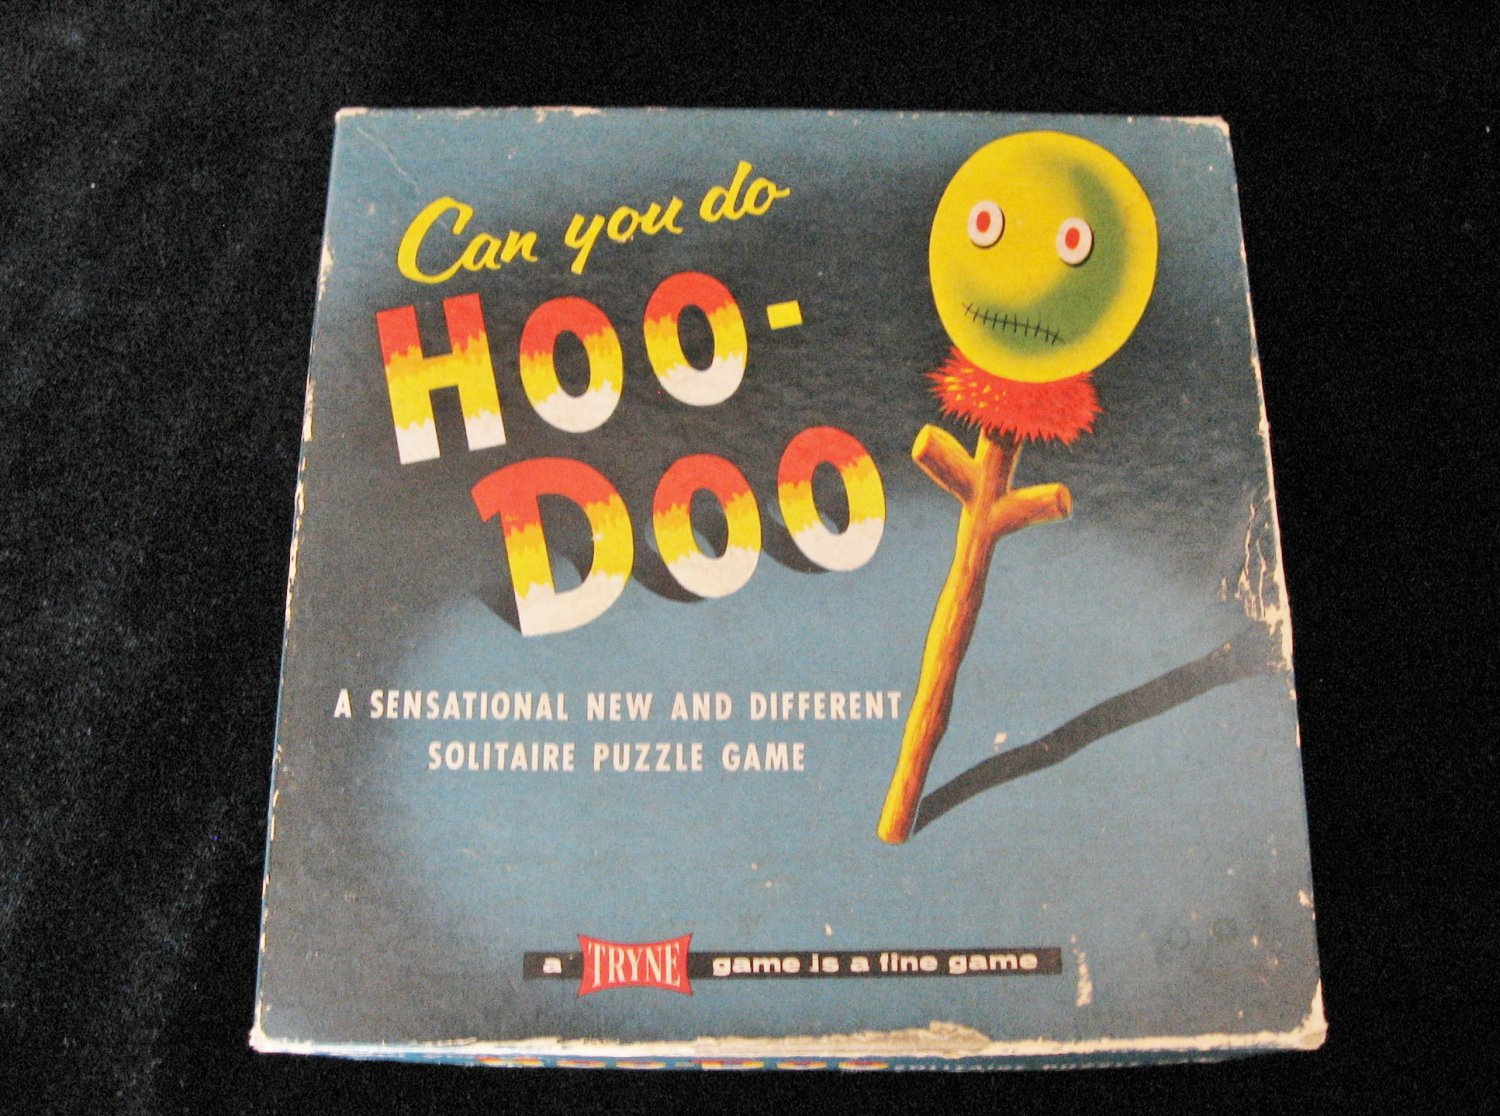
\includegraphics[width=5cm]{hoodoo2.jpg}
    \label{fig:capa original}
}
\quad\quad\quad
\subfloat[Regras]{
    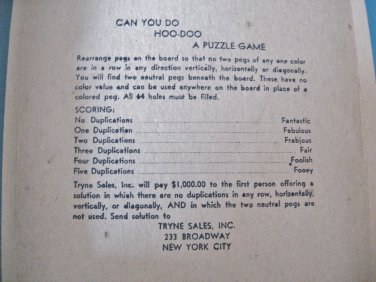
\includegraphics[width=5cm]{regras.jpg}
    \label{fig:regras}
}
\end{figure}

\section{Vari\'{a}veis de Decis\~{a}o}

Para modelar o problema em causa, usamos uma vari\'{a}vel por cada posi\c{c}\~{a}o no tabuleiro, perfazendo para um tabuleiro $n * m$, $n * m$ vari\'{a}veis.O dom\'{i}nio dessas vari\'{a}veis depende tamb\'{e}m ele do tamanho do tabuleiro, sendo que existem para cada tipo de tabuleiro dois dom\'{i}nios distintos dependendo de o jogo ser resolvido usando pe\c{c}as transparentes ou n\~{a}o.
Para o caso de serem usadas pe\c{c}as transparentes o dom\'{i}nio de cada uma das vari\'{a}veis \'{e} $[0,n]$.
No caso de se recorrer somente a pe\c{c}as com cor o dom\'{i}nio de cada uma das vari\'{a}veis passa a ser $[1,n]$.

No caso de o jogo ser resolvido recorrendo aos \emph{pegs} transparentes \'{e} ainda utilizada uma vari\'{a}vel extra, que \'{e} a soma do valor de todas as outras. Na resolu\c{c}\~{a}o do jogo tentar-se-\`{a} minimizar o valor desta vari\'{a}vel que tem um dom\'{i}nio que \'{e} $[0,n^3]$ num tabuleiro de $n * m$ onde n \'{e} a maior dimens\~{a}o. 

\section{Restri\c{c}\~{o}es}

Tratando-se de um jogo todas as restri\c{c}\~{o}es que inclu\'{i}mos s\~{a}o r\'{i}gidas, \`{a} excep\c{c}\~{a}o de uma.
As restri\c{c}\~{o}es r\'{i}gidas s\~{a}o:

\begin{itemize}
\item A restri\c{c}\~{a}o que impede que duas pe\c{c}as da mesma linha tenham valores iguais;
\item A restri\c{c}\~{a}o que impede que duas pe\c{c}as da mesma coluna tenham valores iguais;
\item A restri\c{c}\~{a}o que impede que duas pe\c{c}as da mesma diagonal tenham valores iguais;
\end{itemize}

A restri\c{c}\~{a}o flex\'{i}vel, diz respeito \'{a} tentativa de minimizar o n\'{u}mero de pe\c{c}as transparentes envolvidas na resolu\c{c}\~{a}o do tabuleiro (que \'{e} por si tamb\'{e}m um dos objectivos do jogo).

A implementa\c{c}\~{a}o das restri\c{c}\~{o}es r\'{i}gidas \'{e} feita agrupando as vari\'{a}veis em listas, ora por linha, ora por coluna, ora por diagonal , e chamando o predicado \emph{all\_distinct} sobre essas listas, obrigando assim que nunca hajam duas pe\c{c}as que partilhem a mesma linha/coluna/diagonal que tenham o mesmo valor.

A implementa\c{c}\~{a}o da restri\c{c}\~{a}o flex\'{i}vel, \'{e} feita pela introdu\c{c}\~{a}o de uma vari\'{a}vel antes do \emph{labeling}, a qual se passa ao predicado \emph{sum} para que represente a soma do valor de todas as vari\'{a}veis do tabuleiro. Ap\'{o}s a aplica\c{c}\~{a}o desta restri\c{c}\~{a}o o \emph{labeling} \'{e} chamado dentro do \emph{min}, permitindo assim obter a solu\c{c}\~{a}o cuja soma dos valores das pe\c{c}as \'{e} maior, valor esse que necess\'{a}riamente inclui o menor n\'{u}mero poss\'{i}vel de pe\c{c}as transparente (pe\c{c}as com o valor zero).

\section{Estrat\'{e}gia de Pesquisa}
%
A estrat\'{e}gia utilizada para a etiquetagem das vari\'{a}veis foi tentar atribuir valores primeiro, \'{a}quelas que est\~{a}o mais restritas por forma a tenta minimizar a \'{a}rvore de pesquisa, "cortando" n\'{o}s o mais cedo poss\'{i}vel. Isto \'{e} conseguido usando a op\c{c}\~{a}o \emph{ffc} que tenta atribuir valores primeiro \'{a}s vari\'{a}veis com um dom\'{i}nio menor, sendo que o crit\'{e}rio de desempate seleciona a vari\'{a}vel com mais restri\c{c}\~{o}es suspensas.


\section{Visualiza\c{c}\~{a}o}

Existem seis predicados utilizados para a construção visual do tabuleiro em modo de texto. O primeiro predicado a ser executado é o \textit{print\_tab(+board)} que recebe como argumento um tabuleiro representado por uma lista de listas de inteiros. Este predicado calcula o comprimento da lista, e das sub-listas. Obtidos os números de linhas e colunas do tabuleiro em questão, procede-se à impressão. Enquanto a cauda da lista não for vazia, isto é, ainda existirem mais linhas, segue-se um procedimento básico, que consiste em imprimir primeiro uma linha horizontal, numa nova linha verificar o tamanho do índice, para calcular o número de caracteres vazios a escrever entre o índice e início do tabuleiro(este processo de escalonamento do espaço para alinha a impressão também é usado para os valores das pegs no interior do tabuleiro), e só de seguida é impressa a linha de valores, que é a primeira lista. Este ciclo repete-se até chegar então à situação onde a cauda da lista é vazia. 
\paragraph*{}
Quando a cauda da lista é vazia, a primeira parte do processo mantém-se(impressão da linha horizontal, e também dos valores com o respectivo alinhamento), mas após a impressão dos valores da lista, é de imediato impressa outra linha horizontal e seguida do índice das colunas com valores Alfa-numéricos. 
Vemos em baixo um exemplo de tabuleiro impresso na consola:
\paragraph*{}


\begin{figure}[h!]
\begin{center}
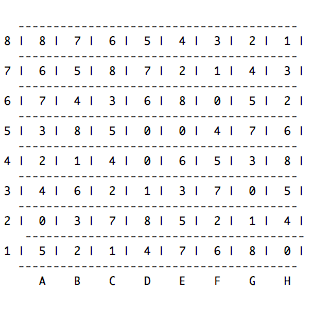
\includegraphics[scale=0.6]{tabuleiro.png}
\caption{\textit{Tabuleiro 8x8 resolvido}}
\label{fig:jogo_original}
\end{center}
\end{figure}







\section{Resultados}



\section{Conclus\~{o}es}

(TODO: A espera dos resultados)


\end{document}